%%%%%%%%%%%%%%%%%%%%%%%%%%%%%%%%%%%%%%%%%%%%%%%%%%%%%%%%%%%%%%%%%%%%%
%% This is a (brief) model paper using the achemso class
%% The document class accepts keyval options, which should include
%% the target journal and optionally the manuscript type. 
%%%%%%%%%%%%%%%%%%%%%%%%%%%%%%%%%%%%%%%%%%%%%%%%%%%%%%%%%%%%%%%%%%%%%
\documentclass[journal=jacsat,manuscript=article]{achemso}

%%%%%%%%%%%%%%%%%%%%%%%%%%%%%%%%%%%%%%%%%%%%%%%%%%%%%%%%%%%%%%%%%%%%%
%% Place any additional packages needed here.  Only include packages
%% which are essential, to avoid problems later. Do NOT use any
%% packages which require e-TeX (for example etoolbox): the e-TeX
%% extensions are not currently available on the ACS conversion
%% servers.
%%%%%%%%%%%%%%%%%%%%%%%%%%%%%%%%%%%%%%%%%%%%%%%%%%%%%%%%%%%%%%%%%%%%%
\usepackage[version=3]{mhchem} % Formula subscripts using \ce{}
\usepackage{tabularx}
\usepackage[usenames,dvipsnames]{xcolor}

%%%%%%%%%%%%%%%%%%%%%%%%%%%%%%%%%%%%%%%%%%%%%%%%%%%%%%%%%%%%%%%%%%%%%
%% If issues arise when submitting your manuscript, you may want to
%% un-comment the next line.  This provides information on the
%% version of every file you have used.
%%%%%%%%%%%%%%%%%%%%%%%%%%%%%%%%%%%%%%%%%%%%%%%%%%%%%%%%%%%%%%%%%%%%%
%%\listfiles

%%%%%%%%%%%%%%%%%%%%%%%%%%%%%%%%%%%%%%%%%%%%%%%%%%%%%%%%%%%%%%%%%%%%%
%% Place any additional macros here.  Please use \newcommand* where
%% possible, and avoid layout-changing macros (which are not used
%% when typesetting).
%%%%%%%%%%%%%%%%%%%%%%%%%%%%%%%%%%%%%%%%%%%%%%%%%%%%%%%%%%%%%%%%%%%%%

%%%%%%%%%%%%%%%%%%%%%%%%%%%%%%%%%%%%%%%%%%%%%%%%%%%%%%%%%%%%%%%%%%%%%
%% Meta-data block
%% ---------------
%% Each author should be given as a separate \author command.
%%
%% Corresponding authors should have an e-mail given after the author
%% name as an \email command. Phone and fax numbers can be given
%% using \phone and \fax, respectively; this information is optional.
%%
%% The affiliation of authors is given after the authors; each
%% \affiliation command applies to all preceding authors not already
%% assigned an affiliation.
%%
%% The affiliation takes an option argument for the short name.  This
%% will typically be something like "University of Somewhere".
%%
%% The \altaffiliation macro should be used for new address, etc.
%% On the other hand, \alsoaffiliation is used on a per author basis
%% when authors are associated with multiple institutions.
%%%%%%%%%%%%%%%%%%%%%%%%%%%%%%%%%%%%%%%%%%%%%%%%%%%%%%%%%%%%%%%%%%%%%

\author{Michael Weinold}
\email{mweinold@ethz.ch}
\affiliation[PSI]{Technology Assessment Group, Paul Scherrer Institute, Villigen, Switzerland}
\alsoaffiliation[ETHZ]
{Chair for Entrepreneurial Risk, ETH Zurich, Zurich, Switzerland}
\alsoaffiliation[UCAM]
{Cambridge Centre for Environment, Energy and Natural Resource Governance, Department of Land Economy, University of Cambridge, Cambridge, United Kingdom}


\author{Sergey Kolesnikov}
\affiliation[UCAM]
{Cambridge Centre for Environment, Energy and Natural Resource Governance, Department of Land Economy, University of Cambridge, Cambridge, United Kingdom}


\author{Laura Diaz Anadon}
\affiliation[UCAM]{Cambridge Centre for Environment, Energy and Natural Resource Governance, Department of Land Economy, University of Cambridge, Cambridge, United Kingdom}
\alsoaffiliation[UHarv]
{Belfer Center for Science and International Affairs, Harvard University, Cambridge MA, USA}

%%%%%%%%%%%%%%%%%%%%%%%%%%%%%%%%%%%%%%%%%%%%%%%%%%%%%%%%%%%%%%%%%%%%%
%% The document title should be given as usual. Some journals require
%% a running title from the author: this should be supplied as an
%% optional argument to \title.
%%%%%%%%%%%%%%%%%%%%%%%%%%%%%%%%%%%%%%%%%%%%%%%%%%%%%%%%%%%%%%%%%%%%%
\title[]{Rapid technological progress in white light-emitting diodes and its sources in innovation and technology spillovers}

%%%%%%%%%%%%%%%%%%%%%%%%%%%%%%%%%%%%%%%%%%%%%%%%%%%%%%%%%%%%%%%%%%%%%
%% Some journals require a list of abbreviations or keywords to be
%% supplied. These should be set up here, and will be printed after
%% the title and author information, if needed.
%%%%%%%%%%%%%%%%%%%%%%%%%%%%%%%%%%%%%%%%%%%%%%%%%%%%%%%%%%%%%%%%%%%%%
\abbreviations{IR,NMR,UV}
\keywords{American Chemical Society, \LaTeX}

%%%%%%%%%%%%%%%%%%%%%%%%%%%%%%%%%%%%%%%%%%%%%%%%%%%%%%%%%%%%%%%%%%%%%
%% The manuscript does not need to include \maketitle, which is
%% executed automatically.
%%%%%%%%%%%%%%%%%%%%%%%%%%%%%%%%%%%%%%%%%%%%%%%%%%%%%%%%%%%%%%%%%%%%%
\begin{document}

%%%%%%%%%%%%%%%%%%%%%%%%%%%%%%%%%%%%%%%%%%%%%%%%%%%%%%%%%%%%%%%%%%%%%
%% The "tocentry" environment can be used to create an entry for the
%% graphical table of contents. It is given here as some journals
%% require that it is printed as part of the abstract page. It will
%% be automatically moved as appropriate.
%%%%%%%%%%%%%%%%%%%%%%%%%%%%%%%%%%%%%%%%%%%%%%%%%%%%%%%%%%%%%%%%%%%%%

%%%%%%%%%%%%%%%%%%%%%%%%%%%%%%%%%%%%%%%%%%%%%%%%%%%%%%%%%%%%%%%%%%%%%
%% The abstract environment will automatically gobble the contents
%% if an abstract is not used by the target journal.
%%%%%%%%%%%%%%%%%%%%%%%%%%%%%%%%%%%%%%%%%%%%%%%%%%%%%%%%%%%%%%%%%%%%%
\begin{abstract}
  The first commercial white light-emitting diodes (LEDs) were introduced to the market in 1996. Since then, white LEDs have experienced major improvements in performance and efficiency. Significant decreases in cost have been driven by a rapid expansion of the market share of LED-based solid-state lighting (SSL), which in turn has driven down costs even further. Today, the technology is one of the key solutions in global climate change mitigation efforts. However, despite its significance, the extent and sources of the underlying improvements have not been systematically investigated. Understanding what has driven rapid progress in LEDs can provide lessons for accelerating innovation in a broad range of other demand-side clean energy technologies. With this aim, we gather and analyse systematic evidence on cost and performance improvements in white LEDs from cost and performance modelling, augmented by a literature review and interviews with experts in industry and academia. We find that the overall efficiency of the highest performing warm white LED packages has improved from $\eta_L=5.8\%$ in 2003 to $\eta_L=38.8\%$ in 2020. During the same period, we estimate that the cost of manufacturing low-power and mid-power LED packages at a U.S. location using state-of-the-art equipment has dropped from 1.1\$ to 0.05\$ (in 2020 USD) between 2003 and 2020, a 95.5\% decrease. We further show that technology spillovers — i.e., knowledge originating in other technologies, sectors, or scientific disciplines — affected all performance dimensions of LEDs, contributing no less than 8.5\% to total efficiency improvements and $\sim$100\% to the improvements in consumer experience metrics identified, thereby playing a key role in the widespread adoption of the technology. The increase in wafer size and manufacturing yield improvements were the primary causes of LED manufacturing cost reductions.
\end{abstract}

%%%%%%%%%%%%%%%%%%%%%%%%%%%%%%%%%%%%%%%%%%%%%%%%%%%%%%%%%%%%%%%%%%%%%
%% Start the main part of the manuscript here.
%%%%%%%%%%%%%%%%%%%%%%%%%%%%%%%%%%%%%%%%%%%%%%%%%%%%%%%%%%%%%%%%%%%%%
\section{Introduction}
\label{sec:intro}

A rapid reduction of global carbon dioxide emissions is urgently required in order to mitigate the effects of climate change \cite{Forster2019}. According to the United Nations, by the end of 2021, more than 130 countries have set or are considering setting a net zero emissions target by 2050 \cite{un2021climate}. The European Union, for example, has set a target of net zero emissions by 2050. It aims to meet this goal with the help of the European Green Deal, alongside other EU and national policies \cite{eu2020green}. The United Kingdom similarly has adopted a national strategy to achieve net-zero by 2050 \cite{noauthor_ieairena_2023}.

Achieving these ambitious and critically important targets will require both the deployment of new clean energy technologies, and the acceleration of innovation in existing supply-side \cite{sinn2012green} and demand-side energy technologies \cite{rgeVorsatz2009}. To ensure rapid adoption of these technologies, significant reductions in their costs and improvements in their performance and consumer experience are needed. This requires understanding how these cost reductions and performance improvements can be achieved \cite{Stephan2021,Ziegler2021}.

There are a range of mechanisms that contribute to improvements in a technology over time, including targeted research and development (R\&D) efforts, economies of scale, learning by doing \cite{Arrow1971}, and economies of scope \cite{johansson2012global,national2016power,iea2020perspectives}. The role of these factors at different stages of the innovation life cycle \cite{ grubler2012policies}, from research and technology development to demonstration, market formation and diffusion, is an area of active research \cite{Mowery1979} \cite{kavlak2018evaluating} \cite{Ziegler2021}. Innovation is also driven by forces of supply and demand. Various \textit{"technology-push"} drivers reduce the costs of innovating, while \textit{"market-pull"} drivers increase the pay-offs from investing in innovation \cite{anadon2009policy}.

The stages and drivers of the innovation life-cycle for a particular technology play out within a broader innovation system \cite{grubler2012policies,Anadon2016}. Among these drivers, the role of external  knowledge transfer and technology spillovers in research and development of energy technologies is an understudied area  \cite{Stephan2021}. While the exact definition of spillovers in the literature depends on the context and the research question \cite{Liu2003,Nemet2012}, we follow Stephan et al. \cite{Stephan2021} and consider knowledge to be external - thus a spillover -  if it has been developed for application in other technologies, sectors, or scientific disciplines. There is emerging evidence that understanding spillovers and the knowledge network outside a technology may be an important factor in understanding \cite{Pichler2020} and shaping \cite{Clark2016,Stephan2021,Sun2021,kolesnikov2022technology} the future evolution of technologies.

Among demand-side technologies, the provision of lighting is a particularly important area for climate change mitigation efforts, as it currently   accounts for 15-19\% of global electricity consumption \cite{Zissis2016,doe_electricity}. It is also an area of rapid recent technological change: since the introduction of the first commercial white light-emitting diodes (LEDs) in 1996, lighting technology has experienced dramatic efficiency improvements.  As shown in Figure \ref{fgr:history_efficacy}, thanks to the introduction of LED-based solid-state lighting (SSL), the efficacy of lighting sources has increased by three orders of magnitude in just over 20 years, which is significantly faster than the historical progress observed in previous lighting technologies \cite{weinold2021quantifying}. For comparison, the highest performing light-emitting devices today reach efficacies of 220 lm/W \cite{lumistrips2021mid}, while an incandescent light bulb can only reach efficacies of up to 18 lm/W. Moreover, this rapid improvement in efficiency has been accompanied by a similarly impressive decrease in LED manufacturing costs and retail prices. Figure \ref{fgr:cost_lamp_small} shows how LED retail prices have fallen by two orders of magnitude, at an annual price per flux decline of 27.3\% during the 2008-2020 period, in line with previous estimates \cite{Gerke2020}.

\begin{figure}[h!]
 \centering
 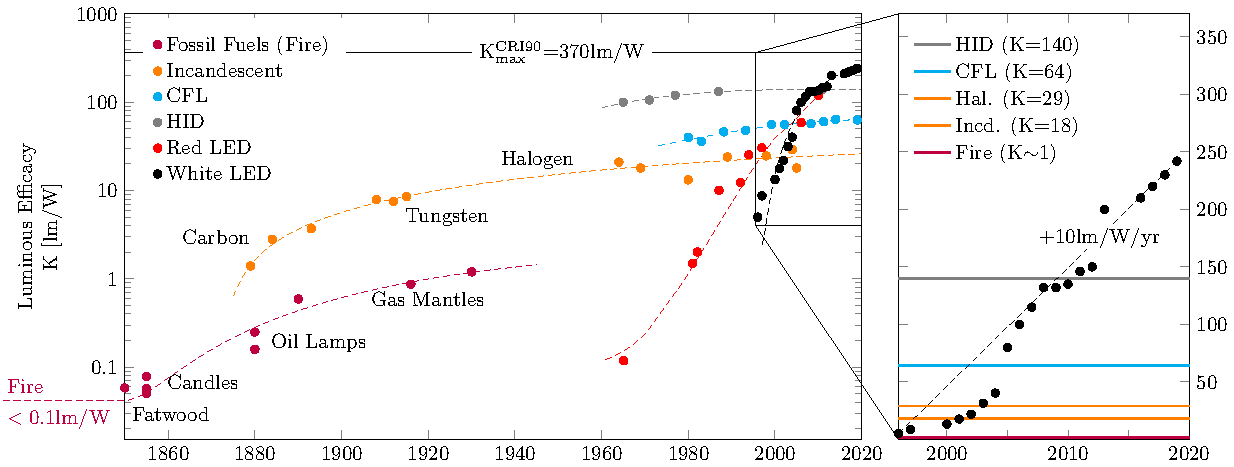
\includegraphics[width=\textwidth]{2_SSL_EST/article/figures/history_efficacy.pdf}
 \caption{Historical development of the luminous efficacy ($K$) of the most widely-used lighting technologies in human history. Data points indicate best performers by year of market introduction. Luminous efficacy is the measure of how efficiently a light source converts electrical energy into visible light that can be perceived by the human eye, taking into account the wavelength sensitivity of the eye (see Supplementary Information, Section 1 for details). Dashed lines indicate an average improvement for each technology, computed from a 3rd-order polynomial fit to the data. The physical limit for an ideal light source with a colour rendering index of CRI=90, denoted as $K_max^{CRI90}$, is shown as a black horizontal line, as per calculations by Murphy et al. \cite{Murphy2012}. The magnified plot shows the progress in cool white LEDs from 1996 to 2020, with the dashed line indicating a linear rate of efficacy improvement of 10lm/W per year. For comparison, efficacies of best performers in legacy lighting technologies for 2020 are shown as coloured horizontal lines. Note the logarithmic scale of the vertical axis on the main plot and the linear scale on the magnified plot. Abbreviations: HID - High-Intensity Discharge; CFL - Compact Fluorescent Lamp; Hal. - Halogen, Incd. - Incandescent. Source: own synthesis of published data based on a visual approach proposed by Azevedo et al. \cite{azevedo2009transition}. See Supplementary Information, Section 4 for the full list of sources and references.}
 \label{fgr:history_efficacy}
\end{figure}

\begin{figure}[h!]
\centering
  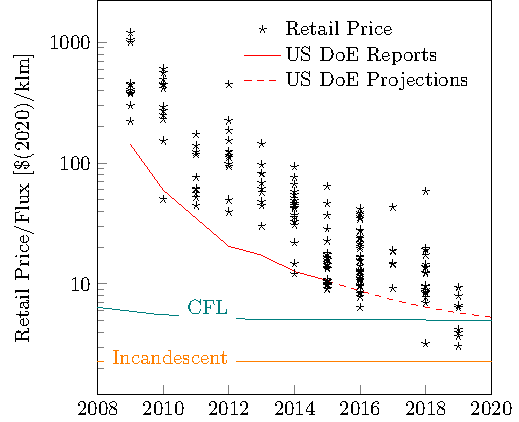
\includegraphics[height=6.5cm]{2_SSL_EST/article/figures/cost_lamp_small.pdf}
  \caption{Historical development of retail sales prices (in 2020 USD) per luminous flux of LED-based luminaires, including light bulbs, spotlights and recessed lights from 2008 to 2020. Red curved and dashed lines represent average retail sales prices and price projections for LED based luminaires published by the U.S. Department of Energy (DOE) \cite{council2013assessment}. Shown for reference are the average prices for compact fluorescent (CFL) and incandescent light bulbs. Source: own synthesis of data on LED sales prices collected from various consumer watchdog databases and publications. Data on CFL sales prices collected from Eger \& Ehlhardt \cite{eger2018origin} as well as various consumer watchdog databases and publications. Incandescent light bulb price is assumed constant based on the average in the covered time period. See Supplementary Information, Section 4, for the full list of sources and references.}
  \label{fgr:cost_lamp_small}
\end{figure}

These dramatic improvements in lighting technology, supported by the introduction of lighting efficiency regulations phasing out incandescent lightbulbs and targeted policies stimulating LED adoption in many countries, led to the rapid expansion and diffusion of SSL technologies  \cite{weinold2020long,Mills2014,Stegmaier2021,grubb2021new}. As a result, by 2020, highly efficient LED luminaires were saving an estimated 131 TWh/year in the EU \cite{eu2019impactass} and 442 TWh/year for the US \cite{guidehouse2020adoption}, which is on par with the amount of energy produced annually by all solar photovoltaic installations in these regions. Notably, market adoption of LED lighting is not limited to developed economies \cite{Kamat2020}. For example, durability, low up-front cost and high efficiency of LED light sources have led to their widespread adoption in rural West African communities without access to grid electricity \cite{Bensch2017}. LEDs have also been used in a wide range of applications beyond lighting, such as personal health monitors \cite{o2019optical,Wyatt2020}, watches and smartphones \cite{Bai2017}, potable water treatment \cite{Lui2014}, high-bandwidth wireless data transmission \cite{Haas2016}, and augmented reality eye wear \cite{Lee2016}. 

Despite this impressive history, the sources of LED innovation have not received as much attention from researchers as innovation in supply-side  energy technologies, such as solar photovoltaics  \cite{kavlak2018evaluating} or wind energy \cite{qiu2012price,jennings2020policy}, or in lithium-ion batteries for transportation \cite{Ziegler2021,Stephan2021}. To the best of our knowledge, no study has comprehensively discussed the sources or extent of progress across various metrics of LED cost or performance since the introduction of first commercial white LED products.  Understanding the extent to which individual innovations and knowledge spillovers  contributed to improvements in LED technology, how this effect compares to other sources of improvements such as economies of scale, and how these innovations occurred (i.e., by what mechanisms and actors) will provide valuable lessons both for other demand-side technologies and overall for accelerating clean energy innovation.

To address these questions, in this paper we identify a set of metrics suitable for tracking the historical progress of LED lighting technology. We then trace device efficiency and cost improvements, as well as changes in relevant consumer experience metrics from the time of introduction of the first commercial warm white LEDs in 2003 to 2020, the year with the most recent data available at the time of writing. Given the proprietary nature of knowledge in the SSL industry, we collect corresponding information using a multi-method approach combining a systematic literature review of scientific literature and industry reports with patent analysis and a series of elite interviews \cite{tansey2009process} with eminent experts from academia, public research institutions and industry. This approach allows us to identify innovations in white LED technology and examine their origins to discern technology spillovers among them. Data on performance improvements associated with individual innovations identified in patents, scientific publications, industry reports, and interviews is then augmented  by our calculations of device efficiency, including contributions of specific spillovers to the overall LED efficiency (see Supplementary Information for more detail). We further calculate LED manufacturing costs using a bottom-up cost model with process-step resolution that we developed. Finally, we discuss what our observations may mean for our understanding of the innovation process in innovation process in LED technology and for broader policy and industry efforts to accelerate clean energy innovation.

\clearpage
\begin{figure}[h!]
 \centering
 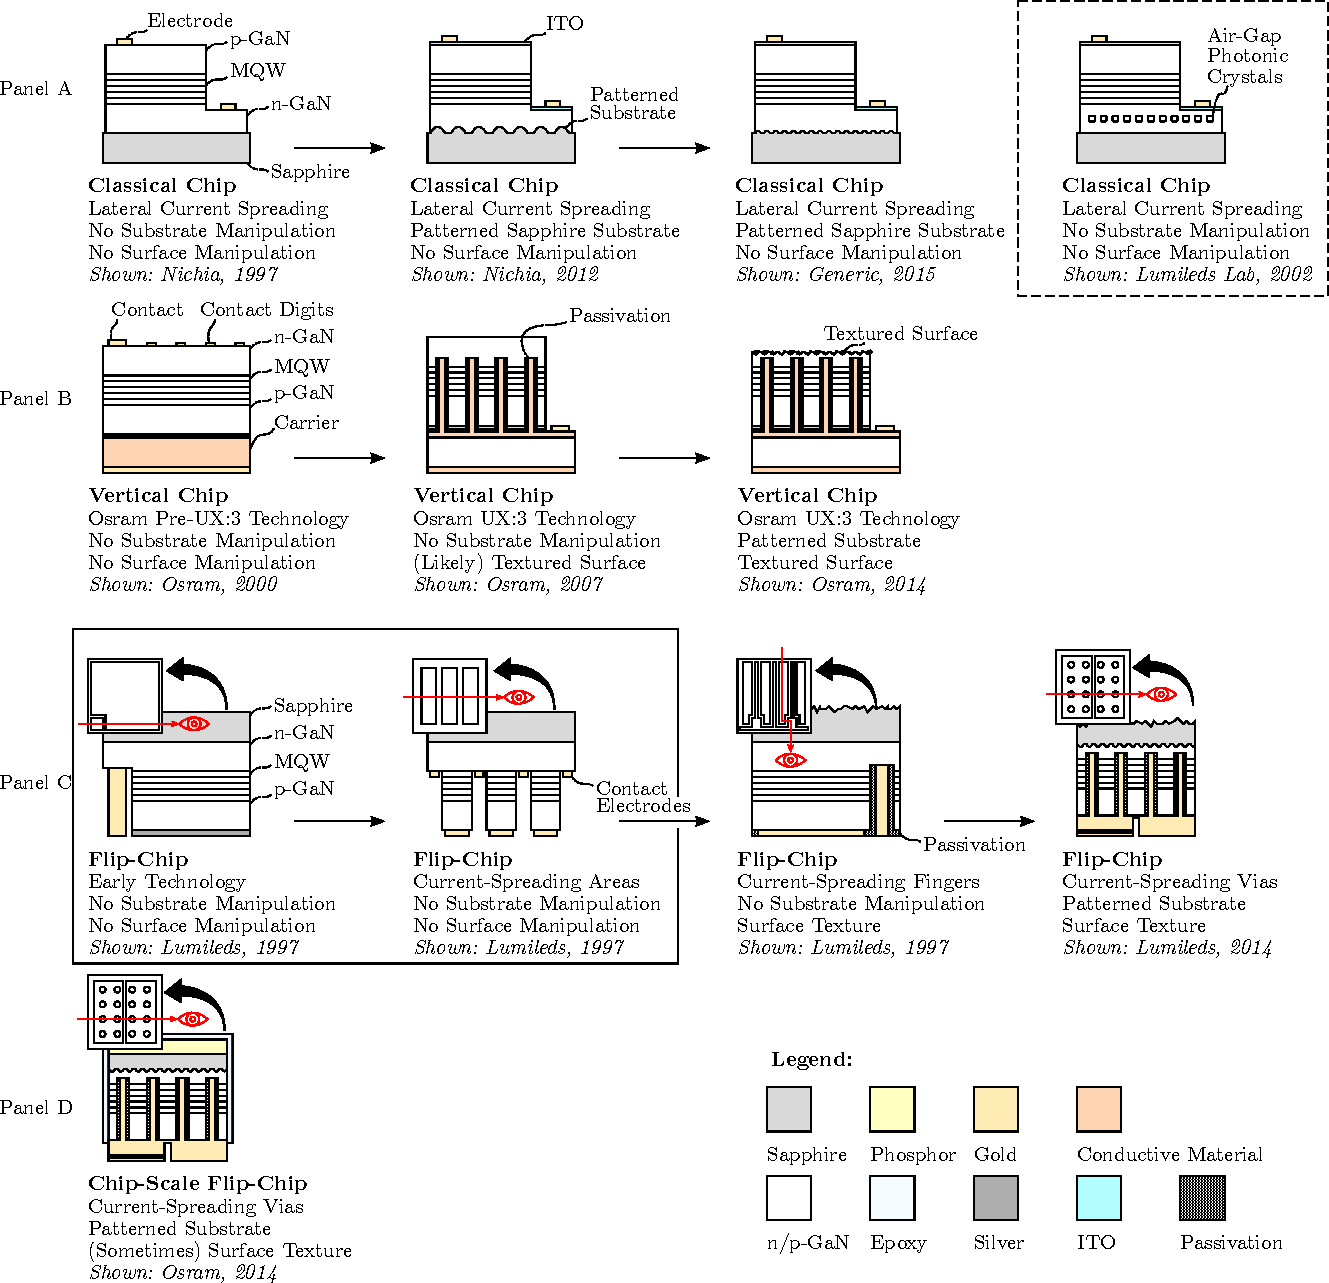
\includegraphics[height=15cm]{2_SSL_EST/article/figures/chip_architecture_overview.pdf}
 \caption{Historical evolution of light-emitting diode chip architectures. Panel A: classical chip with lateral current spreading; Panel B: Osram’s thin GaN flip-chip (vertical) architecture; Panel C: flip-chip architecture; Panel D: chip-scale package flip-chip architecture. Shown are side views of chips without packages, along a cutaway line best suited to the features of each architecture. The cutaway surface is indicated by a red arrow with an eye on the overlaid top view of each chip. Note that the dimensions are not to scale, and smaller features are greatly exaggerated for clarity. Years indicated correspond to the earliest identified patent priority date. Black frames around certain designs indicate chip designs not brought to large-scale production. Chip architecture abbreviations: TF - Thin-Film; FC - Flip-Chip; CSP - Chip-Scale Package; Material abbreviations: GaN - Gallium Nitride, ITO - Indium Tin Oxide, MQW - Multiple Quantum Well. Source: adapted and compiled from multiple patents and industry publications. See Supplementary Information, Section 4, for the full list of sources and references.}
 \label{fgr:chip_architecture_overview}
\end{figure}

\section{Previous Literature}
\label{sec:prev_lit}

The historical development development of light-emitting diodes from a novelty semiconductor experiment into powerful lighting devices has received a considerable amount of attention following the recognition of pioneering work on blue LED by Japanese researchers Shuji Nakamura, Isamu Akasaki and Hiroshi Amano with the 2014 Nobel Prize in Physics \cite{Akasaki2015,Nakamura2015}. The sources and disaggregated contributions of subsequent improvements in LED technology, however, have not been documented in the literature in a systematic fashion, though there were notable publications reporting on the progress in the design of devices \cite{Shchekin2006,krames2007led,laubsch2009high,hahn2014development}, or the technological improvements  underlying the improvement in overall device efficiency for best performers in 2009 \cite{tsao2010solid} and 2016 \cite{pattison2017solid}. 

Several descriptive publications provide a very useful overview of selected scientific breakthroughs that have contributed to LED progress \cite{krames2007status,Phillips2007,Bierhuizen2007,Nakamura2013,feezell2018invention,Taki2019}. Additional studies provide more detail regarding the origin and impact of specific advances in LED technology as well as their integration into device manufacturing were published by authors working for key industry actors Lumileds\cite{MuellerMach2005,Shchekin2006,lumi2015lumi,Bhardwaj2017} and Osram (now amsOsram)\cite{Haerle2004,Baur2009,laubsch2009high,hahn2014development}. However, these studies typically include limited information on the macro-level chip design and cover disparate aspects of the technology over different time periods. Another important source of historical information are patents, which cover the entirety of the device architecture or manufacturing process, including those by Lumileds\cite{margalith2011thin}, Samsung\cite{jung2014phos,cha2019semiconductor} and Soraa\cite{cich2017high}.

We summarize the information collected, analysed and classified on the progress in LED chip architectures and manufacturing processes from these and other disparate sources in Figure \ref{fgr:chip_architecture_overview}, where we show the evolution of LEDs from classical chips with lateral current spreading to chip-scale package flip-chip architectures. Despite the amount of literature published on the topic of LED history, we are not aware of a prior publication that comprehensively and consistently aggregates and analyzes known chip design, manufacturing, and material improvements to show the overall effect of these improvements on device efficiency or manufacturing cost over time. In addition, the effect of individual innovations and technology spillovers, which has been investigated in solar PV \cite{kavlak2018evaluating,kolesnikov2020novel,nemet2019solar}, and to some extent in lithium-ion batteries \cite{Stephan2021}, has not yet been studied in the context of lighting. This is consistent with previous observations regarding the marginalization of end-use technologies in the analysis of energy innovation for climate change impact mitigation \cite{Wilson2012,Creutzig2018}.

\section{Metrics for Technological Progress in LEDs}

Investigating the sources of rapid progress in LED technology over the past decades, in which white LEDs have come to dominate the lighting market \cite{zissis2021}, requires selecting appropriate metrics for tracking and quantifying this progress. The choice of metrics affects both what data sources can be used in the analysis and which research methodologies can be used to calculate and analyse such metrics. We select the metrics based on the following two general criteria. First, we focus only on metrics widely accepted and reported in industry because metrics proposed in the scientific literature but not reported by device manufacturers cannot be used to compare the performance of commercial LED devices over time. Second, the chosen metrics must be useful for understanding the impact of individual technological improvements on relevant performance and cost characteristics.

Historically, the progress in LED technology has commonly be described by pointing to impressive improvements in LED device performance, more specifically device brightness, electrical efficiency and manufacturing cost reductions \cite{Taki2019}. However, metrics related to consumer experience, including the perceived temperature of a white light source and its ability to faithfully render colours, have also played a significant part in the market adoption of new lighting technologies \cite{Menanteau2000,Sandahl2006,CAIRD2008,murphy2012governing} and received substantial attention in LED research and development efforts \cite{azevedo2009transition,cho2017white}. Therefore, a comprehensive analysis of the evolution in white LED technology must take into consideration advances in: 1) physical device performance; 2) consumer experience; and 3) LED device manufacturing costs. Next, we introduce and discuss the metrics that we use to track progress in each of these three areas.

\subsection{Device Performance Metrics}
\label{sec:device_performance_metrics}

During the years following the market introduction of white LEDs, the primary metric of progress in solid-state lighting was typically luminous flux. This was because the luminous flux (total brightness) of early white LEDs was too small to allow for the economical combination of multiple LEDs into lamps for general illumination purposes. In 2000, the highest performing devices yielded around 10lm, just below the output of a candle as defined in the unit candela (1cd=12.57lm)\cite{haitz2011solid}. Progress in this metric was commonly rendered together with the associated reduction in retail prices as “Haitz’s Law”\cite{haitz1999case,haitz2011solid}. Today, however, the devices with the highest performance yield in excess of 1600lm, the equivalent of a 100W incandescent bulb \cite{cree2020bright}. LED brightness has thereby become sufficient to enable the construction of lamps from multiple LED devices, with contemporary improvements focusing instead on higher efficiency and quality of light instead of brightness. Even though a large number of scientific publications and industry periodicals continue to focus on brightness as a metric of progress in lighting, we find that, at this point in time, this metric is insufficient to capture the complexity of the multitude of efficiency improvements that have been driving overall LED efficiency \cite{weinold2021compound}. Specifically, the stagnating levels of luminous flux in the highest performing devices do not capture the outcomes of a major area of LED research, which is improving electrical efficiency at constant brightness.

We therefore use a combination of the total device efficiency ("lamp efficiency") and the sub-efficiencies that describe the different physical loss channels within the device to describe progress in light-emitting diode technology. In line with previous publications \cite{schubert2018light,tsao2010solid}, we use the sub-efficiencies: forward voltage efficiency $\eta_{V_f}$, light extraction efficiency $\eta_{LE}$, internal quantum efficiency $\eta_{IQ}$, droop $\eta_{droop}$, conversion efficiency $\eta_{C}$, spectral efficiency $\eta_{S}$. The equations defining these sub-efficiencies are provided in the Supplementary Information in Section 1.3. The overall efficiency ("Lamp Efficiency") $\eta_L$ of a light-emitting diode package is the product of all considered sub-efficiencies:

\begin{equation}
    \eta_L = \prod_{i=(V_f, \dots, S)} \eta_i
\end{equation}

This metric describes the cumulative electrical and optical losses within the device, as well as the light conversion losses in the phosphor layer.

\subsection{Consumer Experience Metrics}

The perceived quality of light is entirely determined by the emission spectrum of a light source \cite{ies_handbook}. Any metric relevant to customer experience can thus be calculated from the spectrum alone. The spectrum of an LED light source is determined by the emission wavelength of the LED itself and the absorption and emission spectra  of the down-conversion phosphor used in the device. It is typically included in the product datasheets provided by manufacturers, which enables the calculation of all relevant spectrum-based metrics for these devices. Based on the prevalence in scholarly literature and industry publications, for this study we choose two consumer experience metrics: Colour Rendering Index (CRI) and Colour Temperature. We do not consider flicker, the unintended high-frequency temporal modulation of light, which is another important consumer experience metric for lighting and a subject of recent regulation by the European Union \cite{weinold2020long}. This effect is caused not by LEDs themselves, but rather by inadequately designed electrical ballasts \cite{Lehman2014}. As a result, it is beyond the scope of this work. 

\subsubsection{Color Rendering Index (CRI)}

The Colour Rendering Index (CRI) of a light source describes its ability to render the colours of an object faithfully when compared to illumination under a reference light source, such as standard daylight \cite{khan2015led}. The way it is calculated is defined by the International Illumination Commission (CIE) \cite{cie_cri_1995}. CRI has certain limitations when applied to solid-state light sources \cite{david2013cri}. However, despite repeated attempts at constructing more elaborate colour rendering metrics \cite{Houser2013}, CRI has remained the de facto industry standard for describing colour fidelity of light sources \cite{DOE2016LED}. High colour rendering performance of lighting is a requirement in workplace environments, retail stores, clinical operating environments and art exhibitions \cite{khanh2017color}. It should be noted that some niche applications prioritize high colour saturation over high CRI, for instance, in food display or fabric retail applications \cite{david2013cri}. However, these niche applications remain outside our focus on general illumination. Due to a broad availability and importance of CRI data for consumers of various LED lighting sources, we adopt CRI as the key metric to track progress in consumer experience in LED lighting, despite its limitations. 

\subsubsection{Colour Temperature}

The Colour Temperature of a light source describes the equivalent temperature of an ideal black body which emits light of a colour comparable to that of the light source \cite{commission2011cie}. Warm white light sources are widely used in general illumination, while cold white light sources are used in workplace illumination and outdoor lighting. Early white LEDs produced only cool white light \cite{mueller2000light}. The introduction of first commercial warm white LED light bulbs played a significant part in increasing adoption of LED-based lighting among consumers, as their spectrum more closely resembled the warm white colour temperature of incandescent light bulbs \cite{al2016optics}. For this reason, we also adopt colour temperature as a metric for tracking progress in consumer experience in LED lighting.

\subsection{Manufacturing Cost}

In selecting metrics for tracking the progress in manufacturing cost reductions in LED, we must highlight the complexity of this task. Access to manufacturing cost data at the chip level is usually restricted due to its proprietary nature and is available only for selected products. Using sales price information instead of the cost for the same purpose seems a promising alternative, as prices can be easily obtained directly from manufacturers for current products. However, historical data on prices for different chip architectures and different years is similarly difficult to obtain. In addition, sales price includes components not relevant to progress in the technology, such as profit margins and overhead costs, and is affected by policies such as rebates and purchase subsidies. Historical information on these factors and price components, as well as their impact on the manufacturing cost for each LED product under consideration is even harder to obtain, making the use of LED sales prices as a direct metric of technology progress very difficult in practice. 

We address the limitations of data availability for the chip-level LED manufacturing costs and sales prices by developing and applying a bottom-up LED manufacturing cost model with process-step resolution. In our case, it is enabled by the general availability of historical data on prices of relevant raw materials, components, and manufacturing equipment, and the relative cost data on manufacturing processes, which is occasionally published as part of industry press releases \cite{ledinside2013csp}\cite{seoul2015csp}. 

We describe the details of our manufacturing cost model, including its structure and equations, manufacturing process flows for the chip architectures under consideration, input data, explanation of our cost modelling approach based on yielded costs, as well as the model's limitations, in Supplementary Information section 2.4. The model structure is generally based on the 2012 LEDCOM cost model \cite{ledcomv2}, but we expand it significantly both in scope and in its ability to capture historical trends. The model captures three historical time periods corresponding to different “eras” in LED manufacturing: the early period of the first high-power white LEDs around 2003, the period of accelerating consumer adoption of LED lighting around 2012, and the most recent period around 2020, the year of our main data collection efforts. The aggregate result of the cost model is the manufacturing cost per LED package for each of the three years considered, which includes all costs associated with producing the chip, including running costs of the factory.

The cost model we developed and describe in Section 2.4 of the Supplementary Information relies on a cumulative approach to yielded cost\cite{becker2001use}. In this approach, the yielded cost of process step $1$ is defined as the ratio between the total cost of step 1 $C_1$ and the yield of step 1 $Y_1$:

\begin{equation}
    C_{Y_1} = \frac{C_1}{Y_1}, \ C_{Y_2} = C_{Y_{2 \rightarrow 3}} - C_{Y_1} = \frac{C_1(1-Y_2)+C_2}{Y_1Y_2}, \ C_{Y_3}=\dots
\end{equation}

This cost metric is cumulative by definition, thus

\begin{equation}
    \sum_i C_{Y_i} = \frac{\sum_i C_i}{\prod_i Y_i}
\end{equation}

Yielded cost per step is dependent on the step order and blind to downstream information \cite{becker2001use}.

\section{Methods and Data Collection}
\label{sec:methods}

The evolution of LED device architecture and performance as well as the progress in understanding the underlying physical phenomena are well covered in the scholarly literature and patents. However, information provided in such sources is insufficient for our goals on at least three accounts: First, existing work focuses only on selected performance parameters or overall device efficiency, rather than on providing a comprehensive coverage of the whole device sub-efficiencies for a particular LED product or design. Scientific publications also do not always disclose the underlying device architecture or the features responsible for the gains in performance. Second, not all relevant innovations are patented \cite{Pakes_1980,Fontana_2013}. In the case of LED patents in particular, our interviews with industry experts suggest that the propensity to patent is the highest for knowledge related to macroscopic device architecture and chemical composition of phosphors, and the lowest for knowledge related to manufacturing process improvements and microscopic chip architecture that is difficult to reconstruct by reverse engineering. This means that relying only on patent literature would bias results by unduly emphasizing some focus areas and de-emphasizing others. Third, scientific publications and patents typically focus on experimental devices, rather than commercial products. While new LED features, designs and manufacturing methods reported in these sources can potentially result in significant performance gains or cost reductions, it is difficult to ascertain if these improvements have since been adopted in industry.  Furthermore, information on LED manufacturing cost and the effect of process improvements on the total cost is highly proprietary. Estimates are occasionally reported in the scientific literature and company publications, but these often do not disclose which parts of the manufacturing process are responsible for the largest contribution to the overall cost, or which improvements led to cost reductions.

To overcome the limitations of these different methods for understanding technological progress, in this study we rely on a multi-method approach to data collection and analysis, the details of which are provided in Section 2 of the Supplementary Information document. Specifically, we combine information obtained from a systematic review of the primary scientific literature, device datasheets, relevant patents, and industry publications (SI Section 2.1) with information gained from semi-structured interviews with experts from academia and industry (SI Section 2.2), bottom-up manufacturing cost modelling (SI Section 2.3), and our own computations of device sub-efficiencies (SI Section 2.4). We then use this information to track the historical progress in white LED technology over time across the three groups of metrics identified above in the 'Metrics' section and identify its sources in innovation and technology spillovers.

\clearpage
\section{Results}

\subsection{Improvements in Sub-Efficiencies and Overall Efficiency}

The historical development of the sub-efficiencies introduced in Section Device Performance Metrics is shown in Figure SI11 in the Supplementary Information. Using this data, we calculated the overall LED efficiency for four years: 2003, 2010, 2016 and 2020. The waterfall diagrams in Figure \ref{fgr:waterfall} show how improvements in sub-efficiencies led to improvements in the overall white LED lamp efficiency from $\eta_L=5.8\%$ in 2003 to $12.7\%$ in 2010, $32.5\%$ in 2016 and finally to $38.8\%$ in 2020. As is evident from the figure, no single loss channel dominates in terms of its contribution to the overall efficiency, in line with previous observations\cite{tsao2010solid}. We note, however, that the loss channels with a fixed physical limit, e.g., Stokes loss that contributes to the conversion efficiency by phosphors, has become more dominant in 2016 and 2020 compared to 2003 and 2010. This is a direct result of the large efficiency improvements of upstream sub-efficiencies.

Figure \ref{fgr:breakthroughs_efficiency} shows the overall magnitude of contributions of identified LED innovations and technology spillovers to improvements in LED efficiency over time across different sub-efficiencies. The full list of identified LED innovations considered in our study is provided in Table SI2 in Section 3 of the Supplementary Information document. The list of corresponding technology spillovers is provided in Table \ref{tab:spillovers} in the Discussion section below. Through the index decomposition analysis described in Section 2.4 in the Supplementary Information we find that out of the overall LED efficiency increase of 32.9\% from 5.8\% to 38.8\% between 2003 and 2020, at least 2.8\% can be attributed specifically to technology spillovers identified in this study, corresponding to 8.5\% of the total LED efficiency improvements between 2003 and 2020.

In Figure \ref{fgr:breakthroughs_efficiency} we also compare, for the first time, efficiency improvements across sub-efficiencies over time, contrasting them with the physical limits of the corresponding loss channels. We find that there has been consistent progress across all device sub-efficiencies in the recorded period. Specifically, between 2003 and 2020, forward voltage efficiency increased from 70\% to 99.5\%, internal quantum efficiency from 55\% to 90\%, electrical droop from 65\% to 90\%, light extraction efficiency from 60\% to 90\%, spectral efficiency from 74\% to 83\%, conversion efficiency (red) from 11\% to 45\%, conversion efficiency (green) from 19\% to 61\%. Notably, some sub-efficiencies for the most recent devices considered in our study are now within $\sim10\%$ of their respective physical limits. The exception is spectral efficiency which, at $\sim17\%$ below the physical limit, shows larger potential for further improvements.

\begin{figure}[h!]
 \centering
 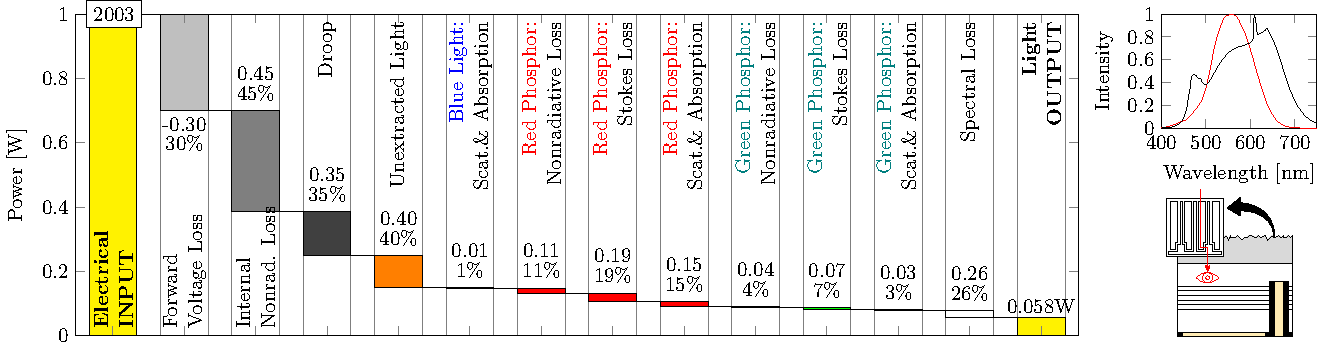
\includegraphics[width=15.5cm]{2_SSL_EST/article/figures/waterfall_performance_2003.pdf}
 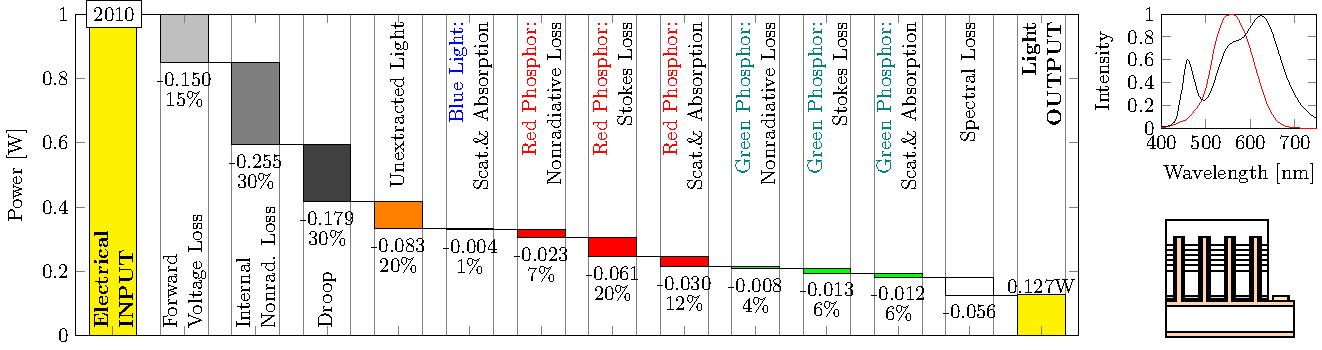
\includegraphics[width=15.5cm]{2_SSL_EST/article/figures/waterfall_performance_2010.pdf}
 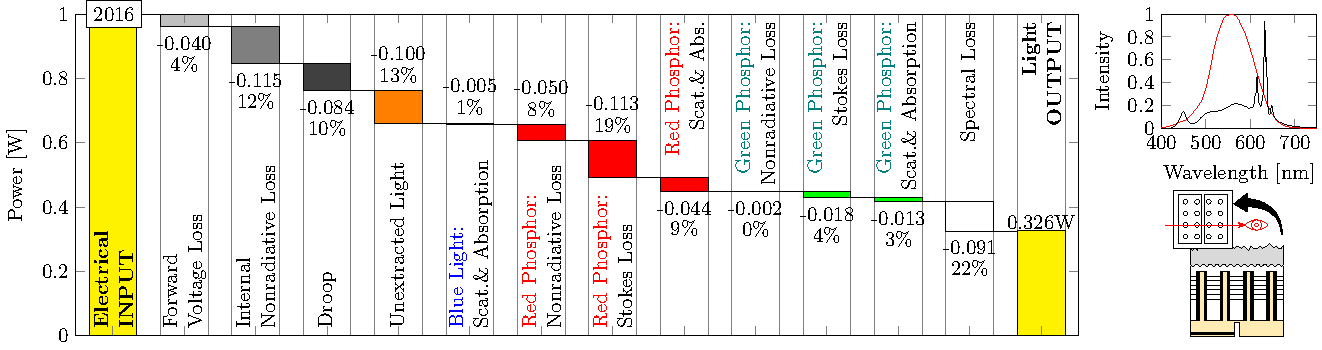
\includegraphics[width=15.5cm]{2_SSL_EST/article/figures/waterfall_performance_2016.pdf}
 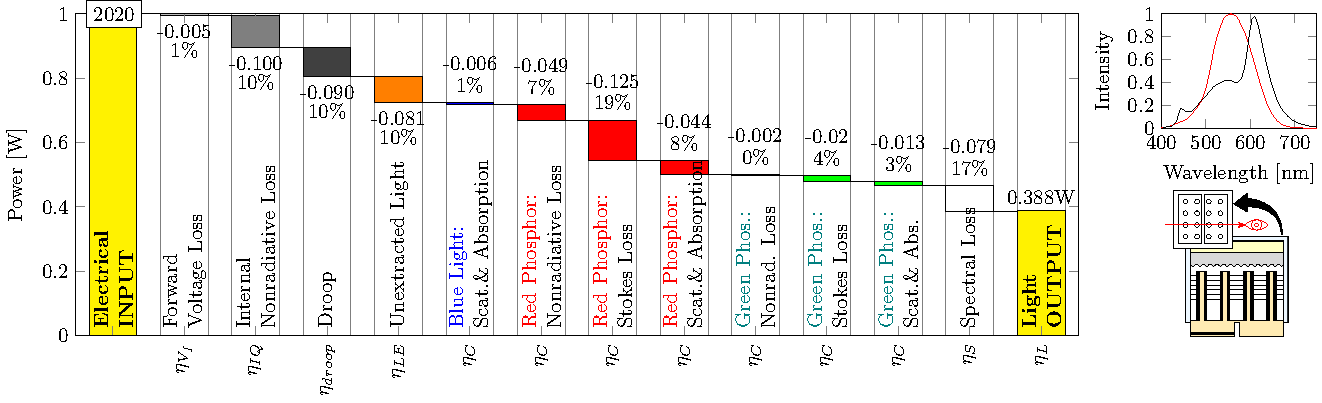
\includegraphics[width=15.5cm]{2_SSL_EST/article/figures/waterfall_performance_2020.pdf}
 \captionsetup{font=footnotesize}
 \caption{Waterfall diagrams of the loss channels in a generic mid/high-power LED package for 2003, 2010, 2016 and 2020 (top to bottom panels), normalized to 1 Watt of electric power input (yellow bar on the left). Sub-efficiencies corresponding to each loss channel are listed below each column and described in Section 1.3 of the Supplementary Information. Numbers for each loss channel indicate energy losses both in relative terms of input power (in percent) at the point of the channel and absolute values (in Watts). Percentages for red, green and blue loss channels indicate losses of remaining red/green/blue light energy. The corresponding LED architectures and associated down-conversion phosphors are shown for reference: 2003 - flip-chip with YGAG phosphor; 2010 - flip-chip with 258 phosphor; 2016 - flip-chip with PFS phosphor; 2020 - flip-chip with SALON phosphor. A more complete overview of LED chip architectures is provided in Figure \ref{fgr:chip_architecture_overview}. Details on phosphor chemical composition are provided in Table \ref{tab:phosphors} with additional data on the spectral performance and invention history provided in Section 3 in the Supplementary Information. Overall LED package efficiency is $\eta_L = 5.8\%$ in 2003, $\eta_L = 12.7\%$ in 2010, $\eta_L = 32.6\%$ in 2016 and $\eta_L = 38.8\%$ in 2010. Abbreviations: Scat. = Scattering. Source (Efficiency): own elaboration based on data in Figure SI11. Source (spectral data): Adapted from publications on the respective phosphors: YGAG (2003)\cite{Mueller2002}, 258 (2010)\cite{MuellerMach2005}, PFS (2016)\cite{Murphy2015}, SALON (2019)\cite{Hoerder2019}.}
 \label{fgr:waterfall}
\end{figure}

\begin{figure}[h!]
 \centering
 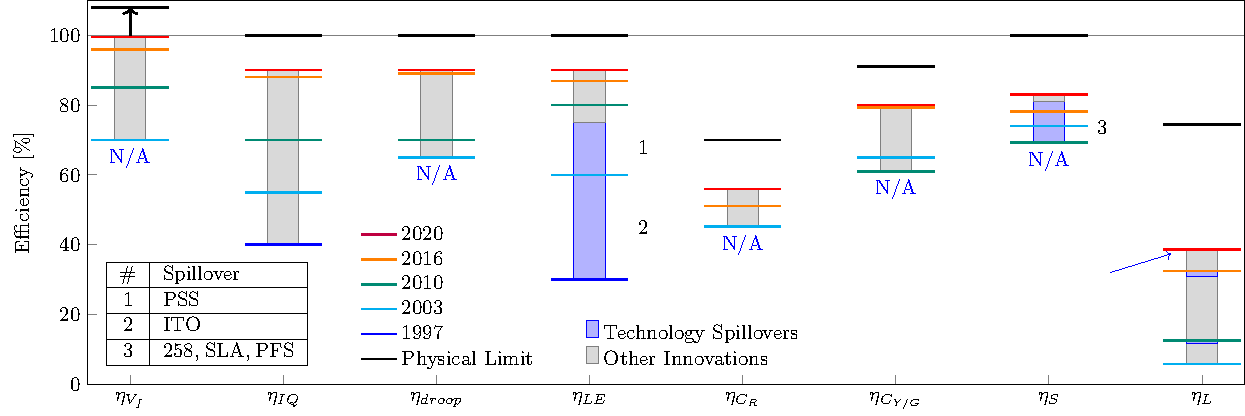
\includegraphics[width=\textwidth]{2_SSL_EST/article/figures/breakthroughs_efficiency.pdf}
 \caption{Contribution of innovations and technology spillovers to the historical progress in sub-efficiencies of phosphor-converted warm white LEDs with test currents of at least 350mA. Vertical bars represent LED technology innovations, with purple bars indicating innovations driven by technology spillovers (annotated and listed in an inset table) and grey bars indicating all other improvements identified in this study. Horizontal coloured lines indicate state-of-the-art sub-efficiency levels for the four years used in Figure \ref{fgr:waterfall}: 2003, 2010, 2016, and 2020. To provide additional historical context, data for 1997 is included for selected sub-efficiencies. "N/A" denotes sub-efficiencies where 1997 data could not be calculated to different reasons: $\eta_{Vf}$, $\eta_{droop}$ depend on the device current, which was below 350mA in 1997, making comparison with contemporary devices difficult. $\eta_{C(R)}$,$\eta_{C(Y/G)}$ and $\eta_S$ are relevant only to warm white spectrum LEDs, which were not available in 1997. Note: ITO current spreading layer affects different sub-efficiencies in different chip architectures, e.g., in modern flip-chip architectures light extraction efficiency no longer depends on ITO, see Figure \ref{fgr:chip_architecture_overview}. Physical limits on sub-efficiencies are indicated by black horizontal lines. The overall LED lamp efficiency, $\eta_L$, is displayed in the rightmost column. $\eta_{V_f}$ - forward voltage efficiency; $\eta_IQ$ - internal quantum efficiency; $\eta_Droop$ - efficiency droop; $\eta_{LE}$ - light extraction efficiency; $\eta_{C(R)}$ - conversion efficiency for red phosphors; $\eta_{C(Y/G)}$ - conversion efficiency for yellow/green phosphors; $\eta_S$ - spectral efficiency; PSS - patterned sapphire substrate, ITO - indium tin oxide current spreading layer; 258, SLA, PFS - different phosphors used in white LEDs, see Table \ref{tab:phosphors}.  Note that physical limit on $\eta_{V_f}$ is above 100\% due to quantum effects which depends on electrical device parameters \cite{david2016electrical}. Source: own elaboration based on data represented in Figure \ref{fgr:waterfall} and Figure SI11 in the Supplementary Information, as detailed in Section Methods and Data Collection.}
 \label{fgr:breakthroughs_efficiency}
\end{figure}

\subsection{Improvements in Consumer Experience Metrics}

Historical improvements in consumer experience metrics for phosphor-converted warm white LEDs are shown in Figure \ref{fgr:consumer_experience}. In general illumination applications, a high colour rendering index (CRI) in combination with a specific, tunable range of possible colour temperatures is desirable. Both metrics are determined by LED device spectra, which, in turn, depend on the properties of the down-conversion materials in the device. We were thus able to establish the links between all major improvements in the two consumer experience metrics identified in this study and individual LED inventions associated either with phosphors or quantum dots. The list of these inventions is provided in Table \ref{tab:spillovers}, while the detailed descriptions of these inventions and corresponding device spectra are provided in Section 3 in the Supplementary Information.

Notably, from detailed descriptions of the history of inventions in this list, which we provide in Section 3.2.2 of the Supplementary Information, we find that only a single invention related to LED consumer experience improvements was originally developed specifically for application in solid-state lighting: the 2016 SALON phosphor compound \cite{seibald2019phosphor,Hoerder2019}. All other inventions in the list were either originally developed for non-LED applications or prominently used knowledge from areas of science and technology beyond LED or SSL. We discuss the details of the corresponding technology spillovers in the Discussion section below.

\begin{table}[h!]
    \footnotesize
    \centering
    \begin{tabularx}{\textwidth}{|l|l|l|X|X|l|}
    \hline
        \textbf{Year} & \textbf{Desig.} & \textbf{Chemical formula} & \textbf{Description} & \textbf{Significance} & \textbf{SI Sec.} \\ \hline
        1996 & YAG & $Y_3 Al_5 O_{12}:Ce$ & Yttrium aluminium garnet (YAG) phosphor activated with cerium & First LED phosphor, enabled white LEDs & SI 5.1.1 \\ \hline
        1996 & YGAG & $(Y_{1-x} Gd_x)_3 Al_5 O_{12}:Ce$ & Gadolinium-doped YAG phosphor & First red-shifted phosphor, enabled warm white LEDs & SI 5.1.1 \\ \hline
        2002 & 258 & $(Ba,Sr)_2 Si_5 N_8:Eu^{2+}$ & Europium-doped nitridosilicate phosphor & First red LED phosphor & SI 5.1.2 \\ \hline
        2003 & QD & N/A & Quantum dot-based phosphor & First use of QD for LED light down conversion & SI 5.1.4 \\ \hline
        2005 & PFS & $K_2 SiF_6: Mn^{4+}$ & Manganese-activated potassium fluorosilicate (PFS) phosphor & First ultra-narrow-band red LED phosphor & SI 5.1.3 \\ \hline
        2013 & SLA & $Sr[Li Al]_3 N_4 ]:Eu^{2+}$ & Europium-doped cuboidal nitridolithoaluminate phosphor & Improved narrow-band red phosphor & SI 5.1.2 \\ \hline
        2016 & SALON & $Sr[Li_2 Al_2 O_2 N_2]:Eu^{2+}$ & Europium-doped oxonitride phosphor & High-performance ultra-narrow-band red phosphor & SI 5.1.2 \\ \hline
    \end{tabularx}
    \caption{LED down-conversion materials (phosphors and quantum dots) related to improvements in consumer experience metrics identified in this study. The \textit{Year} column represents the earliest reported application of invention in white LEDs. These differ from the years used in Figure \ref{fgr:consumer_experience} which correspond to the earliest publication of spectral data for representative LED products that relied on those materials. The \textit{SI Sec.} column refers to the corresponding section in the Supplementary Information that contains references and a detailed description of the history of corresponding invention. Abbreviations: Desig. - Designation, Sec. - Section.}
    \label{tab:phosphors}
\end{table}

\begin{figure}[h!]
 \centering
 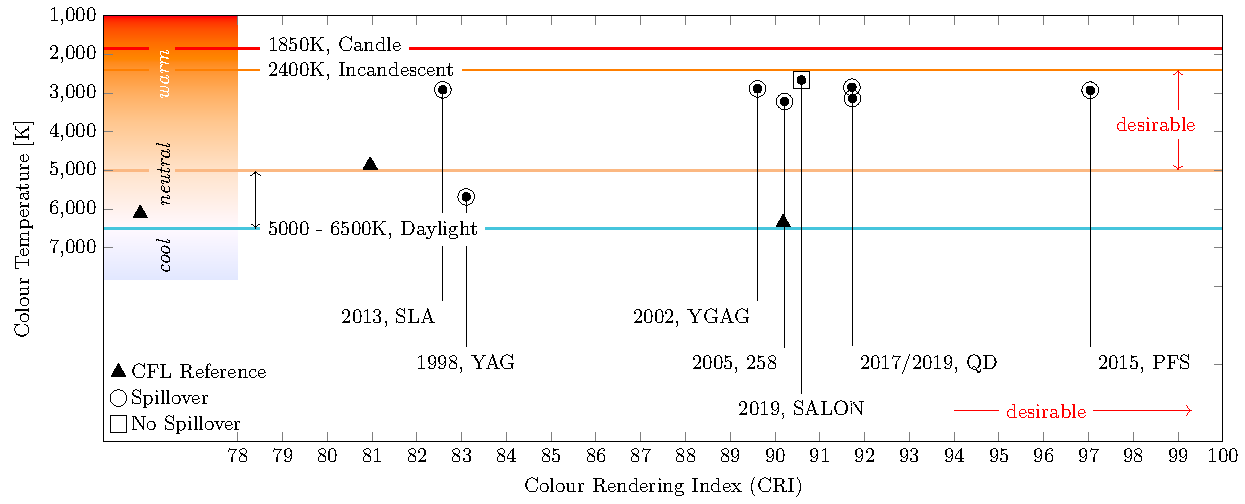
\includegraphics[width=\textwidth]{2_SSL_EST/article/figures/breakthroughs_consumer-experience.pdf}
 \caption{Historical improvements in consumer experience metrics of phosphor-converted white LEDs. Data points show the color temperature and colour rendering index performance of the earliest identified representative white LED products with published spectral data that used phosphors listed in Table \ref{tab:phosphors}, each indicated by the phosphor label and publication year. Corresponding spectral data used to calculate colour temperature values is provided in Figure SI 11 in Section 3 of the Supplementary Information. Three data points representing compact fluorescent lamps (CFLs)\cite{cie_reference}, shown as black triangles, are provided for comparison. Horizontal lines represent typical colour temperatures of “traditional” light sources, shown for reference. The desirable range of colour temperatures for home illumination, indicated by a vertical red arrow, lies between two horizontal orange lines representing typical incandescent light and warm daylight colour temperatures. Horizontal red arrow indicates desirable higher values of colour rendering index (CRI). LED products based on the following phosphor innovations from the following LED manufacturers are represented : YAG - Nichia, 1998 \cite{bando1998development}; YGAG - Lumileds, 2002 \cite{Mueller2002}; 258 - Lumileds, 2005 \cite{MuellerMach2005}; SLA - Lumileds, 2014 \cite{Pust2014}; PFS - GE, 2015 \cite{Murphy2015}; QD - Lumileds, 2017 \cite{lumileds2016qd}, Osram, 2019 \cite{osram2019qd}; SALON - Osram, 2019 \cite{Hoerder2019}.}
 \label{fgr:consumer_experience}
\end{figure}

\subsection{Improvements in Manufacturing Cost}

Figure \ref{fgr:costmodel} shows key results of our manufacturing cost modelling for low-to-mid-power classic chip GaN phosphor-converted white LED packages. We find that the manufacturing cost of a single such LED decreased from 1.11\$ (in 2020 USD) in 2003 to 0.11\$ (2020 USD) in 2012 and 0.05\$ in 2020, a 95.5\% overall decrease.

Among the factors contributing to the LED cost reductions over time, improved manufacturing yields and increases in the wafer size rather than particular LED innovations are found to be responsible for the largest contribution to the overall cost reduction. In the case of manufacturing yield, the higher it is, the less inputs are wasted on the production of a single LED package. With the total manufacturing yield dramatically improving from $\sim25\%$ in 2003 to $\sim75\%$ in 2020 (compare Figure \ref{fgr:costmodel}, Panels A-C), it is not surprising that the total yielded LED manufacturing cost significantly declined over this period. In the case of wafer diameter, the larger the wafer, the more LED chips can be produced from a single wafer. The wafer diameter commonly used in LED manufacturing has been steadily increasing 2003 from 51mm (2 inch) in 2003 to 200mm ($\sim$8 inches, referred to as “8 inch") in 2020. We capture this in the model by assuming the following wafer diameters and calculating the associated number of die per wafer (DPW) \cite{de2005investigation}: $d(2003)\sim 50 mm \rightarrow851 DPW$, $d(2020)\sim200 mm \rightarrow 26,838 DPW$. With more than a thirty-fold increase in the number of die per wafer between 2003 and 2020, the contribution of the whole-of-wafer processing steps to the total cost of manufacturing an individual LED chip and package has dramatically declined over time. As the number of die per wafer increases, the packaging steps, which in the classic chip architecture must be performed separately for each individual LED chip, carry a significantly larger share of the total cost in 2020 than in 2003 (compare Panels A-C in Figure \ref{fgr:costmodel}). However, as our interviewees noted, while growing LEDs on larger wafers is economically desirable, it is associated with engineering and epitaxy challenges as well as high up-front cost of new equipment.

Our findings are further supported by a preliminary sensitivity analysis, presented in Section 2 of the Supplementary Information section, where we find that the sensitivity of the cost model to variation in its main parameters decreases over time with the increase of the number of DPW. We also provide a comparison of our model with past cost calculations and projections published by the US DOE on the basis of the LEDCOM cost model\cite{ledcomv2} and industry data reported to the DOE as part of SSL round tables\cite{doe2010solid}\cite{doe2011solid}\cite{doe2012solid}\cite{doe2013solid}\cite{doe2014solid}\cite{doe2015solid}\cite{doe2016solid} in Section 2 of the Supplementary Information.

\begin{figure*}[h!]
 \centering
 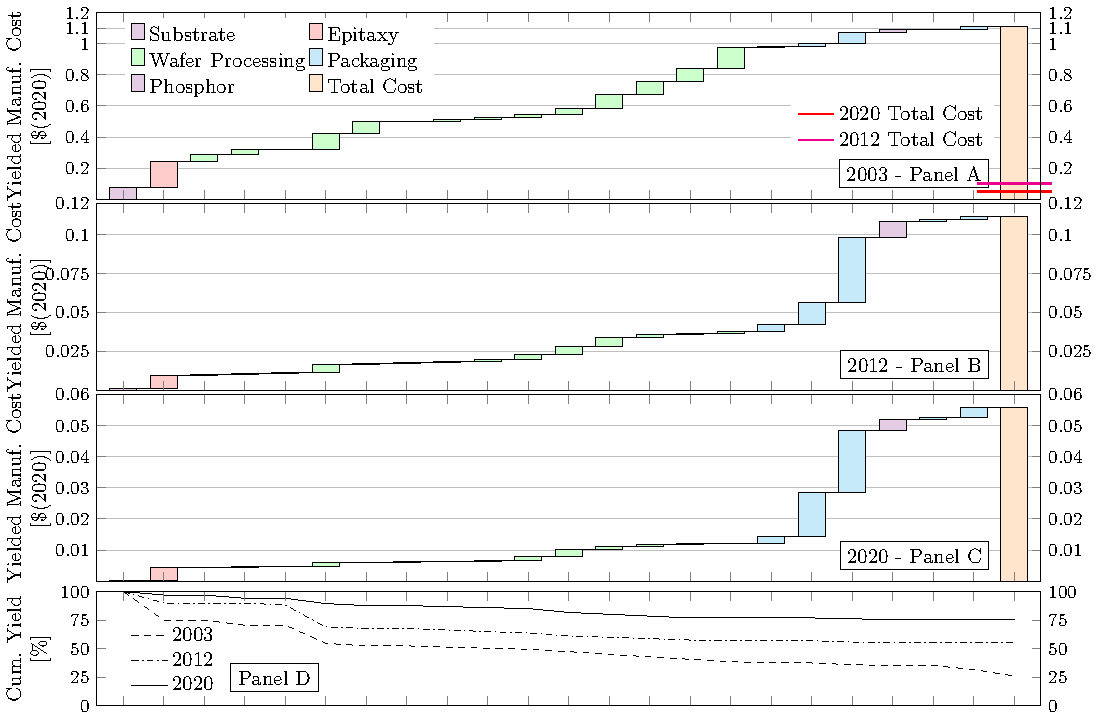
\includegraphics[width=17.5cm]{2_SSL_EST/article/figures/costmodel_results_years.pdf}
 \caption{Manufacturing cost structure modelled for a single low-to-mid power GaN, classic chip, phosphor-converted white LED package, assuming an ideal factory with state-of-the-art equipment at a U.S. location. Consecutive steps shown on the x-axis. Panels A-C: Waterfall diagrams of LED manufacturing cost split by manufacturing process steps for years 2003, 2012 and 2020. Process steps on the horizontal axis are sequenced from left to right in the same order as in the modelled LED manufacturing process. Panel F: Cumulative manufacturing yield after each process step for years 2003, 2012 and 2020. For a visual representation of the overview of the manufacturing process, compare the diagrams in Section 2 of the Supplementary Information. Abbreviations: Litho – Lithographic Process, Insp. – Inspection, Depn. – Deposition, CMP - Chemical-Mechanical Planarization}
 \label{fgr:costmodel}
\end{figure*}

\clearpage
\begin{table}[h!]
    \tiny
    \centering
    \caption{Technology spillovers involved in white LED technology innovations identified in this study.}
    \begin{tabularx}{\textwidth}{|l|l|l|X|X|X|l|X|}
    \hline
        \textbf{Disc.} & \textbf{S/O} & \textbf{Comm.} & \textbf{LED Innovation} & \textbf{Spillover} & \textbf{Origin} & \textbf{Ref.} & \textbf{Area of Improvement} \\ \hline
        1926 & 1994 & 1996 & LED phosphors & Use of phosphors for light down conversion in LEDs & Materials science (S), Cathode ray tubes (T) & \cite{bright1972electric,shimizu1994sheet,cho2017white} & Enabled light down conversion in LEDs \\ \hline
        1967 & 1996 & 1996 & YAG phosphor & Use of YAG phosphor in a first white LED product & Chemistry (S), Materials science (S), Fluorescent lighting (T), Cathode ray tubes (T) & \cite{blasse1967new,bando1996,bando1998development,shimizu1999light,cho2017white} & Enabled white LED products, $\eta_S$, $\eta_C$ \\ \hline
        1967 & 1996 & $<$2002 & YGAG phosphor & Use of YGAG phosphor in first warm white LEDs & Chemistry (S), Materials science (S) &\cite{holloway1969optical,bando1998development,shimizu1999light,Mueller2002} & Enabled warm white LEDs, $\eta_S$, $\eta_C$ \\ \hline
        1982 & 1996 & $<$2010 & Patterned sapphire substrate (PSS) & Use of anti-reflective properties of substrate patterns in LEDs & Optics and photonics (S), Materials science and technology (S,T), Nature-inspired material design (T) &\cite{moharam1982diffraction,krames1998ordered,feezell2018invention,Narukawa_2010} & $\eta_{LE}$, $\eta_{IQ}$ (depending on the chip architecture, compare Figure \ref{fgr:chip_architecture_overview})\\ \hline
        1971 & 1999 & $<$2005 & Indium tin oxide (ITO) current spreading layer & Use of ITO current spreading layer in white LEDs & Optics and photonics (S), Materials science and technology (S,T), Optoelectronic devices (T) & \cite{vossen1971rf,fraser1972highly,margalith1999indium} & $\eta_{Vf}$, $\eta_{LE}$ (depending on the chip architecture, compare Figure \ref{fgr:chip_architecture_overview}) \\ \hline
        1997 & 2002 & 2005 & 258 phosphor & Use of luminescent ‘258’ nitridosilicate compound as LED phosphor & Chemistry (S), Materials science (S) &\cite{Huppertz1997,mueller2004phosphor,MuellerMach2005} & $\eta_S$, $\eta_C$ \\ \hline
        1984 & 2003 & 2009 & Quantum dot-based phosphor & Use of quantum dots for light down conversion in LEDs & Solid-state physics (S), Photochemistry (S), Nanotechnology (T) &\cite{fojtik1984photo,simmonsfinal,ledprof_nexxusqd,bourzac2013quantum} & $\eta_S$, $\eta_C$ \\ \hline
        1972 & 2005 & 2015 & PFS phosphor & Use of knowledge in luminescent materials and skills in "wet" chemical synthesis to synthesize PFS compound and optimize it as LED phosphor & Chemistry (S), Materials science (S) &\cite{paulusz1973efficient,radkov2009red,Murphy2015} & $\eta_S$, $\eta_C$ \\ \hline
        2008 & 2013 & 2015 & SLA phosphor & Use of knowledge about existing cuboidal nitride compounds to identify and synthesize structurally similar SLA phosphor & Structural chemistry (S), Materials science (S), Solid-state physics (S) &\cite{Park2008New,schmidt2013new,Pust2014} & $\eta_S$, $\eta_C$ \\ \hline
    \end{tabularx}
    \begin{tabular}{@{}p{\linewidth}@{}}
        Note: Disc. - Year of initial discovery; S/O - Year of spillover to LED; Comm. - Year of commercial application; Ref. - References. LED innovations are ordered by the year in which a technology spillover into LED occurred, provided in the S/O column. The year of initial discovery is the year of the earliest identified discovery of the original idea or invention outside the LED domain. The year of commercial application is the year of the first recorded application of that idea or invention in a commercial LED product. Origin column represents knowledge domains in which spillovers initially emerged, where (S) denotes a scientific discipline and (T) is an area of technology. Ref. column lists literature sources for the represented innovations and spillovers. Area of Improvement column represents the impact of spillovers on different aspects of white LED technology, e.g., improvements in particular sub-efficiencies.
    \end{tabular}
    \label{tab:spillovers}
\end{table}

\section{Discussion}

\subsection{Performance Improvements}

Our findings show that the overall white LED efficiency has increased from $\eta_L=5.8\%$ in 2003 to $\eta_L=38.8\%$ in 2020. This efficiency increase was predominantly the result of a series of innovations in the LED architecture and materials as well as changes in the manufacturing process. Our comparison of improvements in device sub-efficiencies between 2003 and 2020 shows that the overall efficiency improvement was not dominated by any single sub-efficiency channel. Instead, there has been consistent progress across all device sub-efficiencies during the time period under consideration. Some sub-efficiencies, such as forward voltage efficiency, internal quantum efficiency and light extraction efficiency, are now within $\sim10\%$ of their respective physical limits. A marked trend is the increasing relative contribution of losses in channels with physical limits on efficiency due to the underlying physics, such as light conversion efficiency of phosphors determined by the Stokes shift. Spectral efficiency also remains at $\sim17\%$ from its physical limit, showing potential for further improvements. Research on improving LED performance across efficiency loss channels continues\cite{cho2017white,Weisbuch2020}.

We further find that there has been significant progress in performance across the set of consumer experience metrics, which was driven by innovations related to the conversion of blue light generated by conventional GaN LEDs into the white light required for general illumination. The first commercial white LEDs produced by Nichia in 1996 used a YAG phosphor that could generate only cool white light \cite{bando1998development}. After a series of innovations in phosphors shown in Figure \ref{fgr:consumer_experience} and described in Section 3 of the Supplementary Information, LEDs today can be tuned for high colour rendering performance, high colour saturation and a range of desirable colour temperatures. 

Overall, we find that LED technology innovations made crucial contributions to the progress in both LED performance and consumer experience metrics across the entire period covered by our study. Our interviews have also revealed an important role of incremental process improvements and learning-by-doing\cite{WRIGHT_1936,Arrow_1962} in the progress in LED efficiency. However, further research is needed to quantify the contribution of learning by doing to this progress.

\subsection{Cost Reductions}

Our LED manufacturing cost model shows that the cost of manufacturing low-to-mid power GaN-based white LED packages with classical chip architecture at a U.S. location using state-of-the-art equipment has decreased by 95.5\% from 1.11\$(2020) in 2003 to 0.05\$(2020) in 2020. In contrast with LED performance improvements, where progress was driven mostly by LED technology innovations, the dramatic decline in LED manufacturing cost resulted from an increase in the wafer size used in manufacturing and higher yields across manufacturing steps. This can be seen in the reduction of the contribution of wafer processing steps to  total cost in Figure SI13. Both were enabled by advances in manufacturing equipment performance and incremental process improvements from learning-by-doing.

Notably, our bottom-up cost model is constructed to provide process-step resolution across three different key chip architectures: classical chips, flip chips, and chip-scale package flip chips. However, in this study we were able to collect data and compare the outcomes only for the classical chip architecture. Collecting the full set of data needed to populate the model for the remaining two architectures would require access to proprietary information from industry. With this limitation, tracking manufacturing cost declines across three key LED chip architectures remains a topic for future work.

\subsection{Contribution of Technology Spillovers}
\label{subsec:spillovers}

We find that nine technology spillovers identified in our study, listed in Table \ref{tab:spillovers}, affected all dimensions of white LED performance. Three spillovers associated with the use of YAG/YGAG phosphors in LEDs played the key role in the first commercial white LED lighting products, essentially enabling the solid-state lighting market and industry of today. Spillovers also had a significant effect on physical device performance, cumulatively contributing to 8.5\% of the total LED lamp efficiency improvements between 2003 and 2020. Technology spillovers were particularly important for consumer experience performance of white LED lighting sources, with corresponding spillover-driven innovations responsible for $\sim$100\% of the improvements in consumer experience metrics. 

Following the framework for the analysis of technology spillovers proposed by Stephan and colleagues \cite{Stephan2021}, we gathered information from the interviews, historical records, literature reviews and industry publications to analyze the sources, mechanisms, and enablers of the identified spillovers into the white LED technology listed in Table 4. Among the spillover sources, we find that all nine spillovers had origins in basic science disciplines such as various branches of chemistry, materials science, optics and photonics, and solid-state physics. Five spillovers also utilized technical knowledge and expertise in cathode ray tubes, fluorescent lighting, optoelectronic devices, nanotechnology, and nature-inspired material design. 

Among the spillover mechanisms, six spillovers (involved in all phosphors except PFS and SLA, plus ITO) were a result of application of external scientific and technical knowledge already available to researchers and inventors. Three remaining spillovers (involved in PFS and SLA phosphors, plus PSS) occurred as an outcome of targeted search for relevant external knowledge outside the LED domain. In addition, at least two spillovers (involved in 258 and PFS phosphors) occurred through direct R\&D collaboration.

Among important enabling factors for the identified spillovers, we highlight public mission-driven R\&D funding; industry-academia partnerships; firm experience in multiple industries; conferences that brought together researchers from academia and industry; cultural and language proximity; freedom of search in academia; and university alumni networks.

We find that, on average, it took 26 years from the initial scientific discovery or invention to the moment of its spillover into the LED domain, with this time varying from 5 to almost 70 years. In contrast, it took much less time – just 6 years on average, varying from just a few months to 19 years – to develop a commercial application for the spillover knowledge in the LED market. 

\section{Conclusions}

Our study has analysed the sources of the dramatic cost reductions and performance improvements in white light-emitting diodes since their introduction to the market in 1996 in a systematic and granular way. We find that the total LED device efficiency increase from 5.8\% to 38.8\% between 2003 and 2020, as well as improvements in consumer experience metrics, have been predominantly driven by LED technology innovations that affected all physical energy loss channels and corresponding device sub-efficiencies. We also find that among those innovations, at least nine were driven by knowledge spillovers originating in areas of science and technology beyond LEDs or solid-state lighting. These spillover-driven innovations were responsible for 8.5\% of the total efficiency improvements and nearly 100\% of the improvements in consumer experience metrics. 

Our manufacturing cost model shows a 95.5\% decrease in the cost of producing white classic-chip LEDs (from 1.11\$(2020) to 0.05\$(2020)) between 2003 and 2020, driven mostly by increases in the wafer size and yields across different manufacturing steps over time. In contrast with performance improvements, these cost reductions were thus a result of economies of scale and learning by doing,  which were in turn likely facilitated by policies creating and growing market demand for LED lighting, such as incandescent light bulb bans and subsidies for LEDs.

Our analysis of the sources, mechanisms and enablers of the identified technology spillovers which were significant drivers of improvements in LED efficiency and consumer experience metrics, highlights the critical role played by a deep understanding of the physical, chemical and optical phenomena underlying the operation of LEDs, as well as materials science and technology and nanotechnology involved in the production of LEDs, for past and future advances in LED and solid-state lighting technology. Specifically, deep physical understanding of LED device efficiency loss channels enabled important innovations in LEDs that increased several sub-efficiencies in LEDs and will continue to do so, as expected by eminent experts in the field \cite{Weisbuch2020}. This suggests that additional research in these areas and a more deliberate search for relevant external knowledge may accelerate expected future advances in LED technology. These knowledge spillovers can be enabled or even accelerated by knowledge exchange events and long-term partnerships between academia and industry, dedicated mission-driven public R\&D funding, and a freedom of search in academia. This further reinforces arguments made against the dichotomy of basic research versus applied research \cite{narayanamurti2016cycles,narayanamurti2021genesis} and the calls for open, inclusive and flexible research cultures \cite{Stephan2021}.

There are various important avenues of future research that are opened up by our analysis. First, future work could expand the cost model by collecting and including data for a broader set of chip architectures and analyzing the impact of individual innovations and spillovers on the costs as opposed to performance. Second, a deeper dive on the role of learning-by-doing is needed both in the cost and performance analysis. Third, building on the work on LED sub-efficiencies and physical limits, future efforts could focus on identifying priority areas for further efficiency improvements in LEDs and SSL in general. Finally, by comparing the drivers of innovation, technology spillovers, cost reductions and performance improvements at a granular level across different clean energy technologies, we can identify patterns or differences that would help us formulate recommendations for industry and policymakers aimed at accelerating further clean energy innovation for climate change mitigation. 

%%%%%%%%%%%%%%%%%%%%%%%%%%%%%%%%%%%%%%%%%%%%%%%%%%%%%%%%%%%%%%%%%%%%%
%% The "Acknowledgement" section can be given in all manuscript
%% classes.  This should be given within the "acknowledgement"
%% environment, which will make the correct section or running title.
%%%%%%%%%%%%%%%%%%%%%%%%%%%%%%%%%%%%%%%%%%%%%%%%%%%%%%%%%%%%%%%%%%%%%
\begin{acknowledgement}

This research was supported by the grant from the Alfred P. Sloan Foundation titled \textit{“What factors drive innovation in energy technologies? The role of technology spillovers and government investment”}. Michael Weinold gratefully acknowledges support from the Swiss Study Foundation. The authors thank Venkatesh Narayanamurti, Gabriel Chan, Anna Goldstein, Didier Sornette, and participants of the SPIE West 2021 Conference and C-EENRG Seminar Series of the University of Cambridge for many helpful discussions and feedback. The authors further express their gratitude to all interviewees for their willingness to participate in this study and share their insights. 

\end{acknowledgement}

%%%%%%%%%%%%%%%%%%%%%%%%%%%%%%%%%%%%%%%%%%%%%%%%%%%%%%%%%%%%%%%%%%%%%
%% The same is true for Supporting Information, which should use the
%% suppinfo environment.
%%%%%%%%%%%%%%%%%%%%%%%%%%%%%%%%%%%%%%%%%%%%%%%%%%%%%%%%%%%%%%%%%%%%%
\begin{suppinfo}

Additional context and governing equations of metrics used to quantify progress in solid-state lighting, including the constituent sub-efficiencies of overall lamp efficiency. Detailed description of the multi-method approach used, including the systematic literature review, semic-structured interviews, the manufacturing cost model and performance calculations. Methodological details on dis-aggregation of the contribution of variables to overall lamp efficiency. Additional results, including a breakdown of manufacturing cost and a detailed description of the technology spillovers in phosphor materials for light down-conversion. Complete list of sources for Figures \ref{fgr:chip_architecture_overview} and \ref{fgr:history_efficacy}.

\end{suppinfo}

%%%%%%%%%%%%%%%%%%%%%%%%%%%%%%%%%%%%%%%%%%%%%%%%%%%%%%%%%%%%%%%%%%%%%
%% The appropriate \bibliography command should be placed here.
%% Notice that the class file automatically sets \bibliographystyle
%% and also names the section correctly.
%%%%%%%%%%%%%%%%%%%%%%%%%%%%%%%%%%%%%%%%%%%%%%%%%%%%%%%%%%%%%%%%%%%%%
\bibliography{bibliography}

\end{document}